\subsection{L-shaped bracket}
\label{subsection:l_shaped_bracket}
\paragraph{}
In this example, an L-shaped bracket with isotropic material properties is considered.
Fig.~\ref{iso_fig:l_with_fillet_geo_bc} shows the geometry and the boundary conditions of the problem.
The L-shaped bracket is fixed at one end and subjected to downward vertical displacement at the other end.
Plain strain conditions are assumed.
    \begin{figure}[h!]
        \centering
        \scalebox{0.6}{
            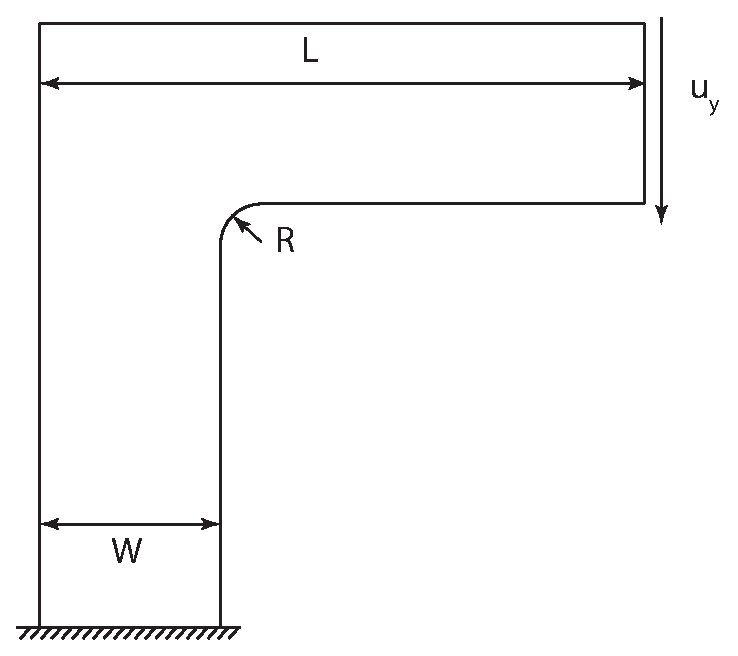
\includegraphics{isogeometric_sbfem/images/l_with_fillet_geo_bc.eps}
        }
        \caption{Geometry and boundary conditions} 
        \label{iso_fig:l_with_fillet_geo_bc}         
    \end{figure}
%
The dimension of the example is: $L=14m$, $W=4m$ and $R=1m$.
While the material properties are: Young's modulus $E=10^3MPa$ and poisson's ratio $\nu=0.3$.
This problem was studied in \citep{LIPTON2010357} by employing the conventional IGA.
In their study, the fillet was modeled as a separate path using biquadratic NURBS with nine control points.

\paragraph{}
In the present study, the control mesh is directly employed for the stress analysis.
However, as the domain does not meet the star convexity, we divide the domain into three subdomains (see Fig.~\ref{iso_fig:l_with_fillet_mesh}).
We employ NURBS to represent the fillet, whilst for the straight lines, we employ Lagrange basis functions.
The results from the present approach are compared with conventional finite element analysis using the commercial
    software ANSYS$^\circledR$.
    \begin{figure}[h!]
        \centering
        \scalebox{0.6}{
            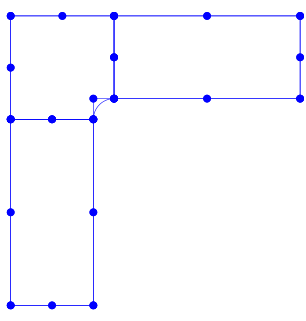
\includegraphics{isogeometric_sbfem/images/l_with_fillet_mesh.png}
        }
        \caption{Control net where `filled' circles represents control points}
        \label{iso_fig:l_with_fillet_mesh}
    \end{figure}
%
\paragraph{}
A total of $2000$ $8$-node quadrilateral elements were used for the finite element analysis.
Fig.~\ref{iso_fig:l_stress_contour} shows the von Mises equivalent stress for the L-shaped bracket with and without the fillet.
As expected, the no fillet case shows higher stress when compared to the L-shaped bracket with the fillet.
From Fig.~\ref{iso_fig:l_stress_contour}, it can be observed that the results from the present approach qualitatively match with the FE solution.
It should be noted that, the proposed method is computationally less intensive than the conventional IGA as it requires
    only the boundary information.
    \begin{figure}[h!]
        \begin{subfigure}[b]{0.5\linewidth}
            \centering
            \scalebox{0.5}{
                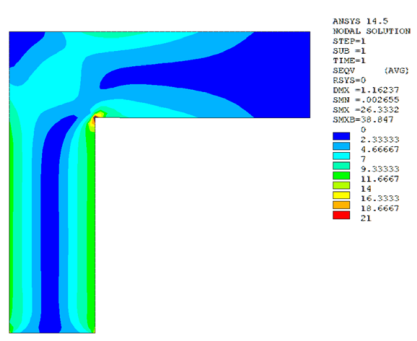
\includegraphics{isogeometric_sbfem/images/l_stress_contour_fem.png}
            }
            \caption{FEM}
        \end{subfigure}
        \begin{subfigure}[b]{0.5\linewidth}
            \centering
            \scalebox{0.5}{
                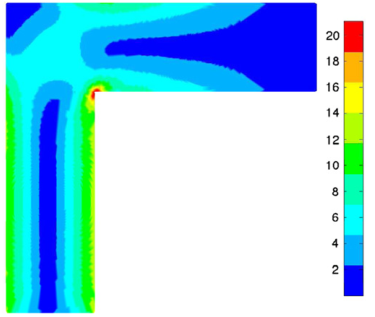
\includegraphics{isogeometric_sbfem/images/l_stress_contour_sbfem.png}
            }
            \caption{Isogeometric SBFEM}
        \end{subfigure}

        \begin{subfigure}[b]{0.5\linewidth}
            \centering
            \scalebox{0.5}{
                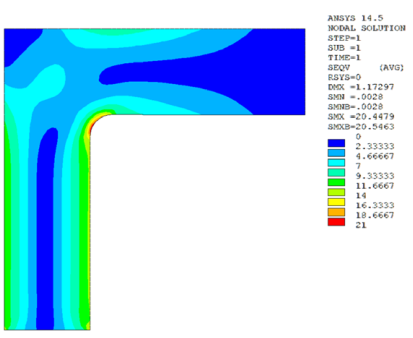
\includegraphics{isogeometric_sbfem/images/l_with_fillet_stress_contour_fem.png}
            }
            \caption{FEM}
        \end{subfigure}
        \begin{subfigure}[b]{0.5\linewidth}
            \centering
            \scalebox{0.5}{
                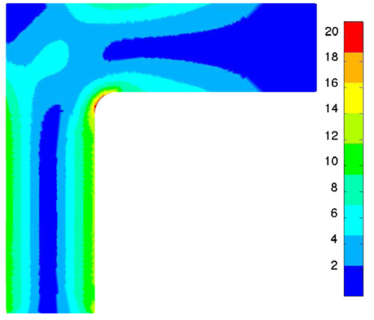
\includegraphics{isogeometric_sbfem/images/l_with_fillet_stress_contour_sbfem.png}
            }
            \caption{Isogeometric SBFEM}
        \end{subfigure}
        \caption{Von Mises equivalent stress contours for L-shaped bracket without and with fillet. The stress values are in Mpa}
        \label{iso_fig:l_stress_contour}
    \end{figure}
%

%=================================================================================================================================%
\paragraph{}
Next, we extend the present formulation to study the transient response of an L-shaped bracket.
The dimensions and the boundary conditions are shown in Fig.~\ref{iso_fig:l_dynamic_geo_bc}.
    \begin{figure}
        \begin{subfigure}[b]{1\linewidth}
            \centering
            \scalebox{0.8}{
                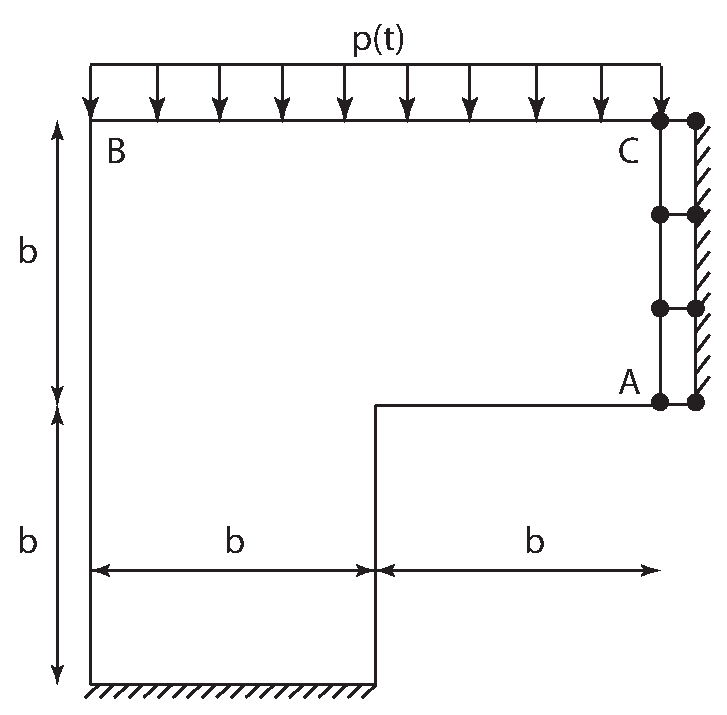
\includegraphics{isogeometric_sbfem/images/l_dynamic_geo_bc.eps}
            }
            \caption{without fillet}
        \end{subfigure}
        \begin{subfigure}[b]{1\linewidth}
            \centering
            \scalebox{0.8}{
                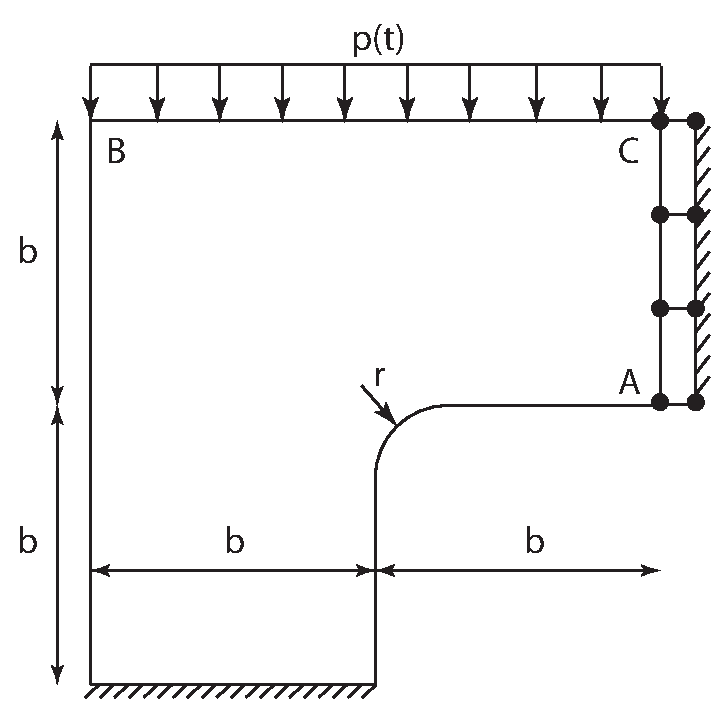
\includegraphics{isogeometric_sbfem/images/l_with_fillet_dynamic_geo_bc.eps}
            }
            \caption{without fillet}
        \end{subfigure}
        \caption{L-shaped bracket: geometry and boundary conditions for transient analysis}
        \label{iso_fig:l_dynamic_geo_bc}
    \end{figure}
%
\paragraph{}
In the example, $b=1m$ and $r=0.2m$.
A state of plane stress is considered and the material properties are:
    Young’s modulus $E = 1 N/m^2$ , poisson’s ratio, $\nu = 1/3$ and mass density, $\rho = 1 kg/m^3$.
    The shear wave velocity is $c_s=\sqrt{3/8}m/s$ and the dilatational wave velocity $c_p=\sqrt{9/8}m/s$
The order of the continued fraction used in Eq.~\ref{lr_eq:sbfem_dynamic_s_full} is chosen as $M_{cf} = 6$.
A uniform pressure $p(t)$ is applied at the side BC of the bracket.
The pressure varies as a triangular impulse in the time domain.
It reaches a peak value $p$ at time $t= 0.5b/c_p$ , reduces to $0$ at $t = b/c_p$ and stays at $0$ afterwards.
The time integration is carried out by using Newmark's method with $\gamma = 1/2$ and $\beta = 1/4$.
The time step is chosen as $\delta t = 0.025b/c_p$.

\paragraph{}
The calculation is performed for 3000 time steps.
For the Isogeometric-SBFEM, the arc is represented with quadratic NURBS functions and the straight lines are discretized with
    Lagrange basis functions.
As the problem domain does not satisfy the star convexity, the domain is sub-divided into three subdomains as done in the static example.
The scaling center for each of the subdomain is placed at the center of the subdomain.
To demonstrate the efficacy of the present formulation, the results are compared with those obtained using the conventional
    finite element method.
A FE mesh leading to a similar accuracy is identified from a convergence study.
The FE analysis is performed with the commercial software ANSYS$^\circledR$ (a total of 2000 8-node quadrilateral elements
    were employed for this study).

\paragraph{}
The vertical displacement responses at point A are plotted in Fig.~\ref{iso_fig:l_uy_dynamic_at_A} as a function of the dimensionless
    time $T = c_pt/b$.
It can be seen that the results from the present formulation agree well with the finite element solution.
    \begin{figure}
        \centering
        \scalebox{0.5}{
            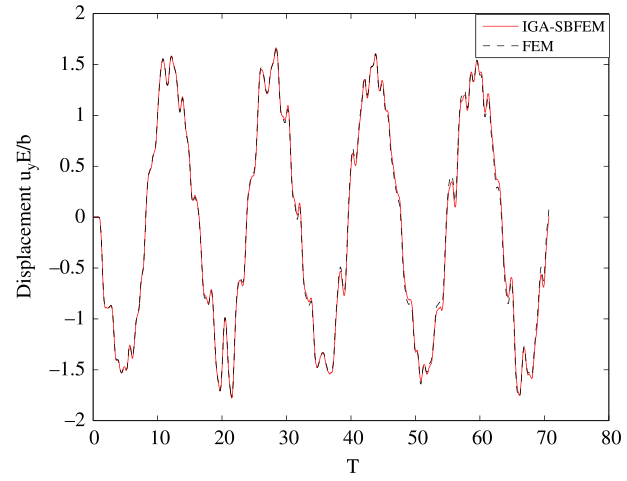
\includegraphics{isogeometric_sbfem/images/l_uy_at_A.png}
        }
    \caption{Vertical displacement of L-shaped bracket at Point A: comparison with conventional FE solution}
    \label{iso_fig:l_uy_dynamic_at_A}
    \end{figure}
%
